% Options for packages loaded elsewhere
\PassOptionsToPackage{unicode}{hyperref}
\PassOptionsToPackage{hyphens}{url}
\PassOptionsToPackage{dvipsnames,svgnames,x11names}{xcolor}
%
\documentclass[
  12pt,
  letterpaper,
  DIV=11,
  numbers=noendperiod]{scrartcl}

\usepackage{amsmath,amssymb}
\usepackage{iftex}
\ifPDFTeX
  \usepackage[T1]{fontenc}
  \usepackage[utf8]{inputenc}
  \usepackage{textcomp} % provide euro and other symbols
\else % if luatex or xetex
  \usepackage{unicode-math}
  \defaultfontfeatures{Scale=MatchLowercase}
  \defaultfontfeatures[\rmfamily]{Ligatures=TeX,Scale=1}
\fi
\usepackage{lmodern}
\ifPDFTeX\else  
    % xetex/luatex font selection
  \setmainfont[Scale = MatchLowercase]{Scala Pro}
  \setsansfont[]{Scala Sans Pro}
\fi
% Use upquote if available, for straight quotes in verbatim environments
\IfFileExists{upquote.sty}{\usepackage{upquote}}{}
\IfFileExists{microtype.sty}{% use microtype if available
  \usepackage[]{microtype}
  \UseMicrotypeSet[protrusion]{basicmath} % disable protrusion for tt fonts
}{}
\makeatletter
\@ifundefined{KOMAClassName}{% if non-KOMA class
  \IfFileExists{parskip.sty}{%
    \usepackage{parskip}
  }{% else
    \setlength{\parindent}{0pt}
    \setlength{\parskip}{6pt plus 2pt minus 1pt}}
}{% if KOMA class
  \KOMAoptions{parskip=half}}
\makeatother
\usepackage{xcolor}
\usepackage[margin=25mm]{geometry}
\setlength{\emergencystretch}{3em} % prevent overfull lines
\setcounter{secnumdepth}{-\maxdimen} % remove section numbering
% Make \paragraph and \subparagraph free-standing
\ifx\paragraph\undefined\else
  \let\oldparagraph\paragraph
  \renewcommand{\paragraph}[1]{\oldparagraph{#1}\mbox{}}
\fi
\ifx\subparagraph\undefined\else
  \let\oldsubparagraph\subparagraph
  \renewcommand{\subparagraph}[1]{\oldsubparagraph{#1}\mbox{}}
\fi


\providecommand{\tightlist}{%
  \setlength{\itemsep}{0pt}\setlength{\parskip}{0pt}}\usepackage{longtable,booktabs,array}
\usepackage{calc} % for calculating minipage widths
% Correct order of tables after \paragraph or \subparagraph
\usepackage{etoolbox}
\makeatletter
\patchcmd\longtable{\par}{\if@noskipsec\mbox{}\fi\par}{}{}
\makeatother
% Allow footnotes in longtable head/foot
\IfFileExists{footnotehyper.sty}{\usepackage{footnotehyper}}{\usepackage{footnote}}
\makesavenoteenv{longtable}
\usepackage{graphicx}
\makeatletter
\def\maxwidth{\ifdim\Gin@nat@width>\linewidth\linewidth\else\Gin@nat@width\fi}
\def\maxheight{\ifdim\Gin@nat@height>\textheight\textheight\else\Gin@nat@height\fi}
\makeatother
% Scale images if necessary, so that they will not overflow the page
% margins by default, and it is still possible to overwrite the defaults
% using explicit options in \includegraphics[width, height, ...]{}
\setkeys{Gin}{width=\maxwidth,height=\maxheight,keepaspectratio}
% Set default figure placement to htbp
\makeatletter
\def\fps@figure{htbp}
\makeatother

\usepackage{fancyhdr}
\usepackage{titling}
\pagestyle{fancy}
\pagenumbering{gobble}
\fancyhf{}
\renewcommand\maketitle{
  \fancyhead[C]{
    \thetitle
    \ifx \theauthor\empty  \else \ – \theauthor \fi
    \ifx \thedate\empty  \else \ – \thedate \ \fi
  }
}
\fancyfoot[C]{\thepage}
\KOMAoption{captions}{tableheading}
\makeatletter
\@ifpackageloaded{caption}{}{\usepackage{caption}}
\AtBeginDocument{%
\ifdefined\contentsname
  \renewcommand*\contentsname{Table of contents}
\else
  \newcommand\contentsname{Table of contents}
\fi
\ifdefined\listfigurename
  \renewcommand*\listfigurename{List of Figures}
\else
  \newcommand\listfigurename{List of Figures}
\fi
\ifdefined\listtablename
  \renewcommand*\listtablename{List of Tables}
\else
  \newcommand\listtablename{List of Tables}
\fi
\ifdefined\figurename
  \renewcommand*\figurename{Figure}
\else
  \newcommand\figurename{Figure}
\fi
\ifdefined\tablename
  \renewcommand*\tablename{Table}
\else
  \newcommand\tablename{Table}
\fi
}
\@ifpackageloaded{float}{}{\usepackage{float}}
\floatstyle{ruled}
\@ifundefined{c@chapter}{\newfloat{codelisting}{h}{lop}}{\newfloat{codelisting}{h}{lop}[chapter]}
\floatname{codelisting}{Listing}
\newcommand*\listoflistings{\listof{codelisting}{List of Listings}}
\makeatother
\makeatletter
\makeatother
\makeatletter
\@ifpackageloaded{caption}{}{\usepackage{caption}}
\@ifpackageloaded{subcaption}{}{\usepackage{subcaption}}
\makeatother
\ifLuaTeX
  \usepackage{selnolig}  % disable illegal ligatures
\fi
\IfFileExists{bookmark.sty}{\usepackage{bookmark}}{\usepackage{hyperref}}
\IfFileExists{xurl.sty}{\usepackage{xurl}}{} % add URL line breaks if available
\urlstyle{same} % disable monospaced font for URLs
\hypersetup{
  pdftitle={Final Exam},
  pdfauthor={Phil 444},
  colorlinks=true,
  linkcolor={black},
  filecolor={Maroon},
  citecolor={Blue},
  urlcolor={Blue},
  pdfcreator={LaTeX via pandoc}}

\title{Final Exam}
\author{Phil 444}
\date{2024-04-26}

\begin{document}
\maketitle

For any question asking for a verbal answer (e.g., explain this notion,
or this constraint), you should answer in about \textbf{250} words.
These are \emph{short answer} questions, not essays, and the aim is to
either (a) simply describe a concept or idea, or (b) present one reason
for or against some notion. Don't try to write a five paragraph essay
for each one. On the other hand, if your answer is much under 250 words,
try explaining a bit more of the background; probably that means that
you are presupposing something that we want you to make explicit.

\begin{enumerate}
\def\labelenumi{\arabic{enumi}.}
\tightlist
\item
  Describe an example where Sen's Condition L (Liberalism) and Condition
  P (Pareto) conflict.
\item
  Describe an example of a \textbf{focal point} in Schelling's sense.
\item
  What is the difference between weak dominance and strict dominance?
  Describe an example where the two notions come apart.
\item
  In Table~\ref{tbl-dom}, what will be the result if both players use
  iterated deletion of strictly dominated strategies to decide what to
  do? (In each cell, Row's payouts are first, and Column's are second.)
\end{enumerate}

\begin{longtable}[]{@{}ccccc@{}}
\caption{Game table for Q4}\label{tbl-dom}\tabularnewline
\toprule\noalign{}
& \textbf{W} & \textbf{X} & \textbf{Y} & \textbf{Z} \\
\midrule\noalign{}
\endfirsthead
\toprule\noalign{}
& \textbf{W} & \textbf{X} & \textbf{Y} & \textbf{Z} \\
\midrule\noalign{}
\endhead
\bottomrule\noalign{}
\endlastfoot
\textbf{A} & 6,3 & 0,4 & 2,7 & 1,3 \\
\textbf{B} & 5,5 & 5,6 & 2,3 & 5,8 \\
\textbf{C} & 2,2 & 3,7 & 7,2 & 3,5 \\
\textbf{D} & 4,7 & 0,4 & 1,6 & 2,2 \\
\end{longtable}

\begin{enumerate}
\def\labelenumi{\arabic{enumi}.}
\setcounter{enumi}{4}
\tightlist
\item
  In Figure~\ref{fig-back}, what will be the result if all players uses
  backward induction to solve the problem? (At each terminal node, the
  payouts are player 1's, then player 2's, then player 3's. Each player
  moves once; first player 1, then player 2, then player 3.)
\end{enumerate}

\begin{figure}

\centering{

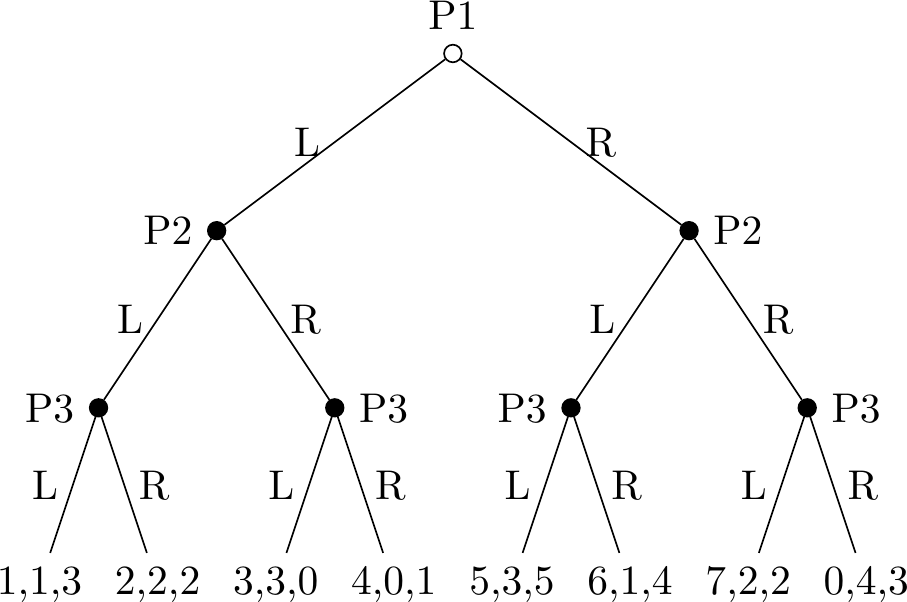
\includegraphics{final_exam_files/figure-pdf/fig-back-1.png}

}

\caption{\label{fig-back}Tree for Q5}

\end{figure}%

\begin{enumerate}
\def\labelenumi{\arabic{enumi}.}
\setcounter{enumi}{5}
\tightlist
\item
  What is the human capital theory of the explanation of the college
  wage premium? Describe one objection to it. (You do not have to answer
  the objection.)
\end{enumerate}



\end{document}
